\documentclass{article} % For LaTeX2e
\usepackage{nips13submit_e,times}
\usepackage{hyperref}
\usepackage{url}
\usepackage{graphicx}
\usepackage{caption}
\usepackage{cite}


\title{RecognizeMyFace\\
\textit{An Exploration of Classifiers for Facial Recognition}}


\author{
Durmus U. Karatay \\
Department of Physics \\
University of Washington \\
\texttt{ukaratay@uw.edu}
\And
Matthias Smith \\ 
Department of Physics \\
University of Washington \\
\texttt{mwsmith2@uw.edu}
}

\nipsfinalcopy
\begin{document}

\maketitle

\begin{abstract}
In this study we explore the effects of using different classifers for recognition of different features after images are processed using Principal Component Analysis (PCA) to reduce dimensionality. We examine five different classifiers, namely, nearest-neighbor (NN), kNN, multivariate Gaussian Mixture Models (GMM), Linear Discriminant Analysis (LDA), and Support Vector Machines (SVM).  After training our model, we selected the best performing classifiers on the validation set for each feature of the images.  We report that different features require different classifiers.
\end{abstract}

\section{Introduction}

We use a well known approach for facial recognition which employs PCA for reducing the dimensionality of the problem.  PCA treats the system as 2-dimensional and projects face images into a face-space that has the information of the variation among the training images. The basis of this face-space is referred to as the eigenfaces.  We try to identify different sets of image features by calculating the projections of eigenfaces onto the images.  We employ five different classifiers after doing a dimensionality reduction with PCA: nearest-neighbor, kNN, multivariate Gaussian Mixture Models, Linear Discriminant Analysis, and Support Vector Machines.

\section{PCA}

Given $N$ images, the $K$ ($\leq N$) most significant eigenfaces can approximate a face. All images are $W \times H$ matrices which are rearranged into $W H \times 1$ column vectors referred to as $\Gamma_i$.  We calculate the average face as

\[
	\Psi = \frac{1}{N} \sum_{i = 1}^{N} \Gamma_i.
\]

We center each face by subtracting off $\Psi$, then we construct the image matrix, $\mathbf{A}$.

\[ 
	\Phi_i = \Gamma_i - \Psi.
\]
\[
	\mathbf{A} = \left[ \Phi_1, \Phi_2, ..., \Phi_N \right].
\]

Since it is computationally expensive to calculate the eigenvectors of such a large matrix, we employ the method described in the original work of Turk et al \cite{tur91}.  

\[
	\mathbf{C} = \mathbf{A} \mathbf{A}^T.
\]

We obtain the eigenvectors of $\mathbf{C}$, $u_i$, by first calculating the eigenvectors of $\mathbf{A^T A}$, namely $v_i$.  

\[
	u_i = \mathbf{A} v_i.
\]

We need to select the most significant $K$ eigenvectors by looking at the eigenvalues.  The variance, $\sigma$ can be used to determine $K$ by selecting a threshold on the fractional variance, $F(\sigma, K)$.

\[
	\sigma = \sum_{i=1}^{N} \lambda_i, \\
\]
\[
	F(\sigma, K) = \frac{\sum_{i=1}^{K} \lambda_i}{\sigma}.
\]

The images in the training set are characterized by calculating the projection of the first $K$ eigenvectors onto the image:

\[
	\omega_{ij} = u_j^T \Phi_i.
\]

For recognition of an unknown image, we center the image by subtracting $\Psi$ and calculate the weight for each eigenface.  With the projected weights we can test against our training set weights to determine the feature.  

\begin{minipage}{\linewidth}
	\centering
	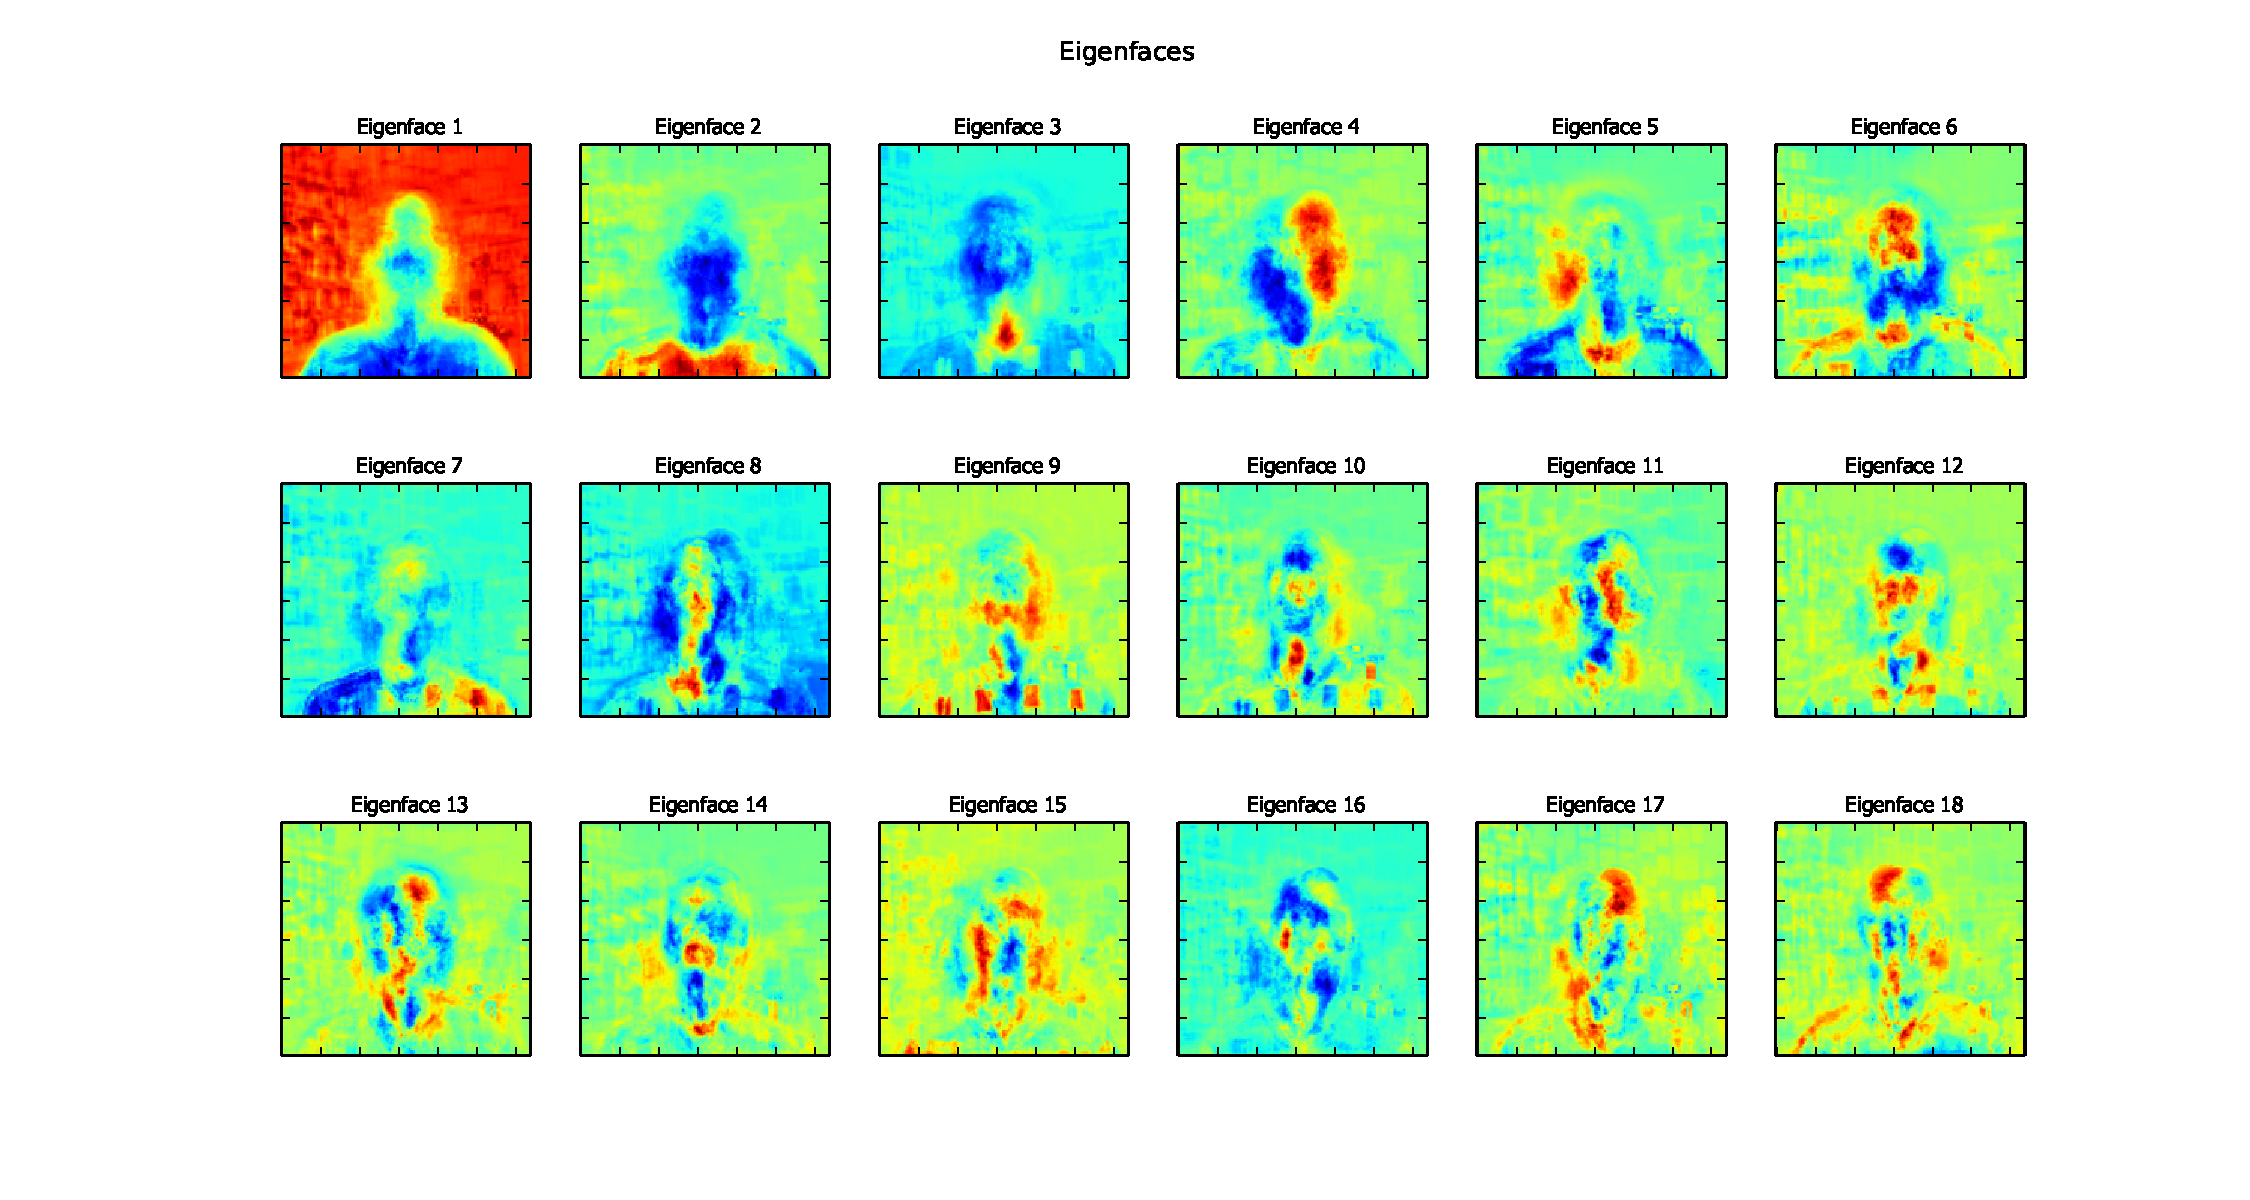
\includegraphics[width=1.0\linewidth]{fig/eigenfaces.pdf}
	\captionof{figure}{The most significant 18 eigenfaces.}
	\label{fig:eigenfaces}
\end{minipage}

\section{Classifiers}

\subsection{Nearest Neighbors}

We employ two different nearest neighbor techniques: Mahalanobis distance and distance weighted kNN.  Mahalanobis distance is defined as\cite{mur12}:

\[
	d(\mathbf{x}, \mathbf{x'}) = \sqrt{(\mathbf{x} - \mathbf{x'})^T \mathbf{C}^{-1} (\mathbf{x} - \mathbf{x'})},
\]

where $\mathbf{C}$ is the covariance matrix of $\mathbf{x}$ and $\mathbf{x'}$.  Mahalanobis distance performs better than Euclidean distance when different dimensions of a vector need different weights, such as the eigenfaces.  This is due to the facts that Mahalonobis distance accounts for the covariance of different dimensions and Euclidean distance suffers from the curse of dimensionality. 

In our kNN implementation we choose $k = 3$ and use distance weighting.  Our kNN uses standard Euclidean distance to find the nearest neighbors.  Even though Euclidean distance suffers from the curse of dimensionality, weighting the neighbors by distance reduces the noise\cite{mur12}.  

\subsection{GMM \& SVM}

We use two clustering techniques, GMM and SVM.  We use both in a semi-supervised fashion with a radial basis function kernel where the kernel is defined as\cite{ski11,mur12}:

\[
	K(\mathbf{x}, \mathbf{x'}) = \exp \left(-\frac{\| \mathbf{x} - \mathbf{x'} \|_2^2}{2 \sigma^2} \right).
\]

\subsection{LDA}

LDA can be used as a classifier with a linear decision boundary.  The decision boundaries are created using class conditional densities from the data. In particular we used LDA with Gaussian densities.  LDA has no parameters to tune, and it is inherently multi-class making it an appropriate choice for separating features with more than two classes\cite{ski11,mur12}.  

\begin{minipage}{\linewidth}
	\centering
	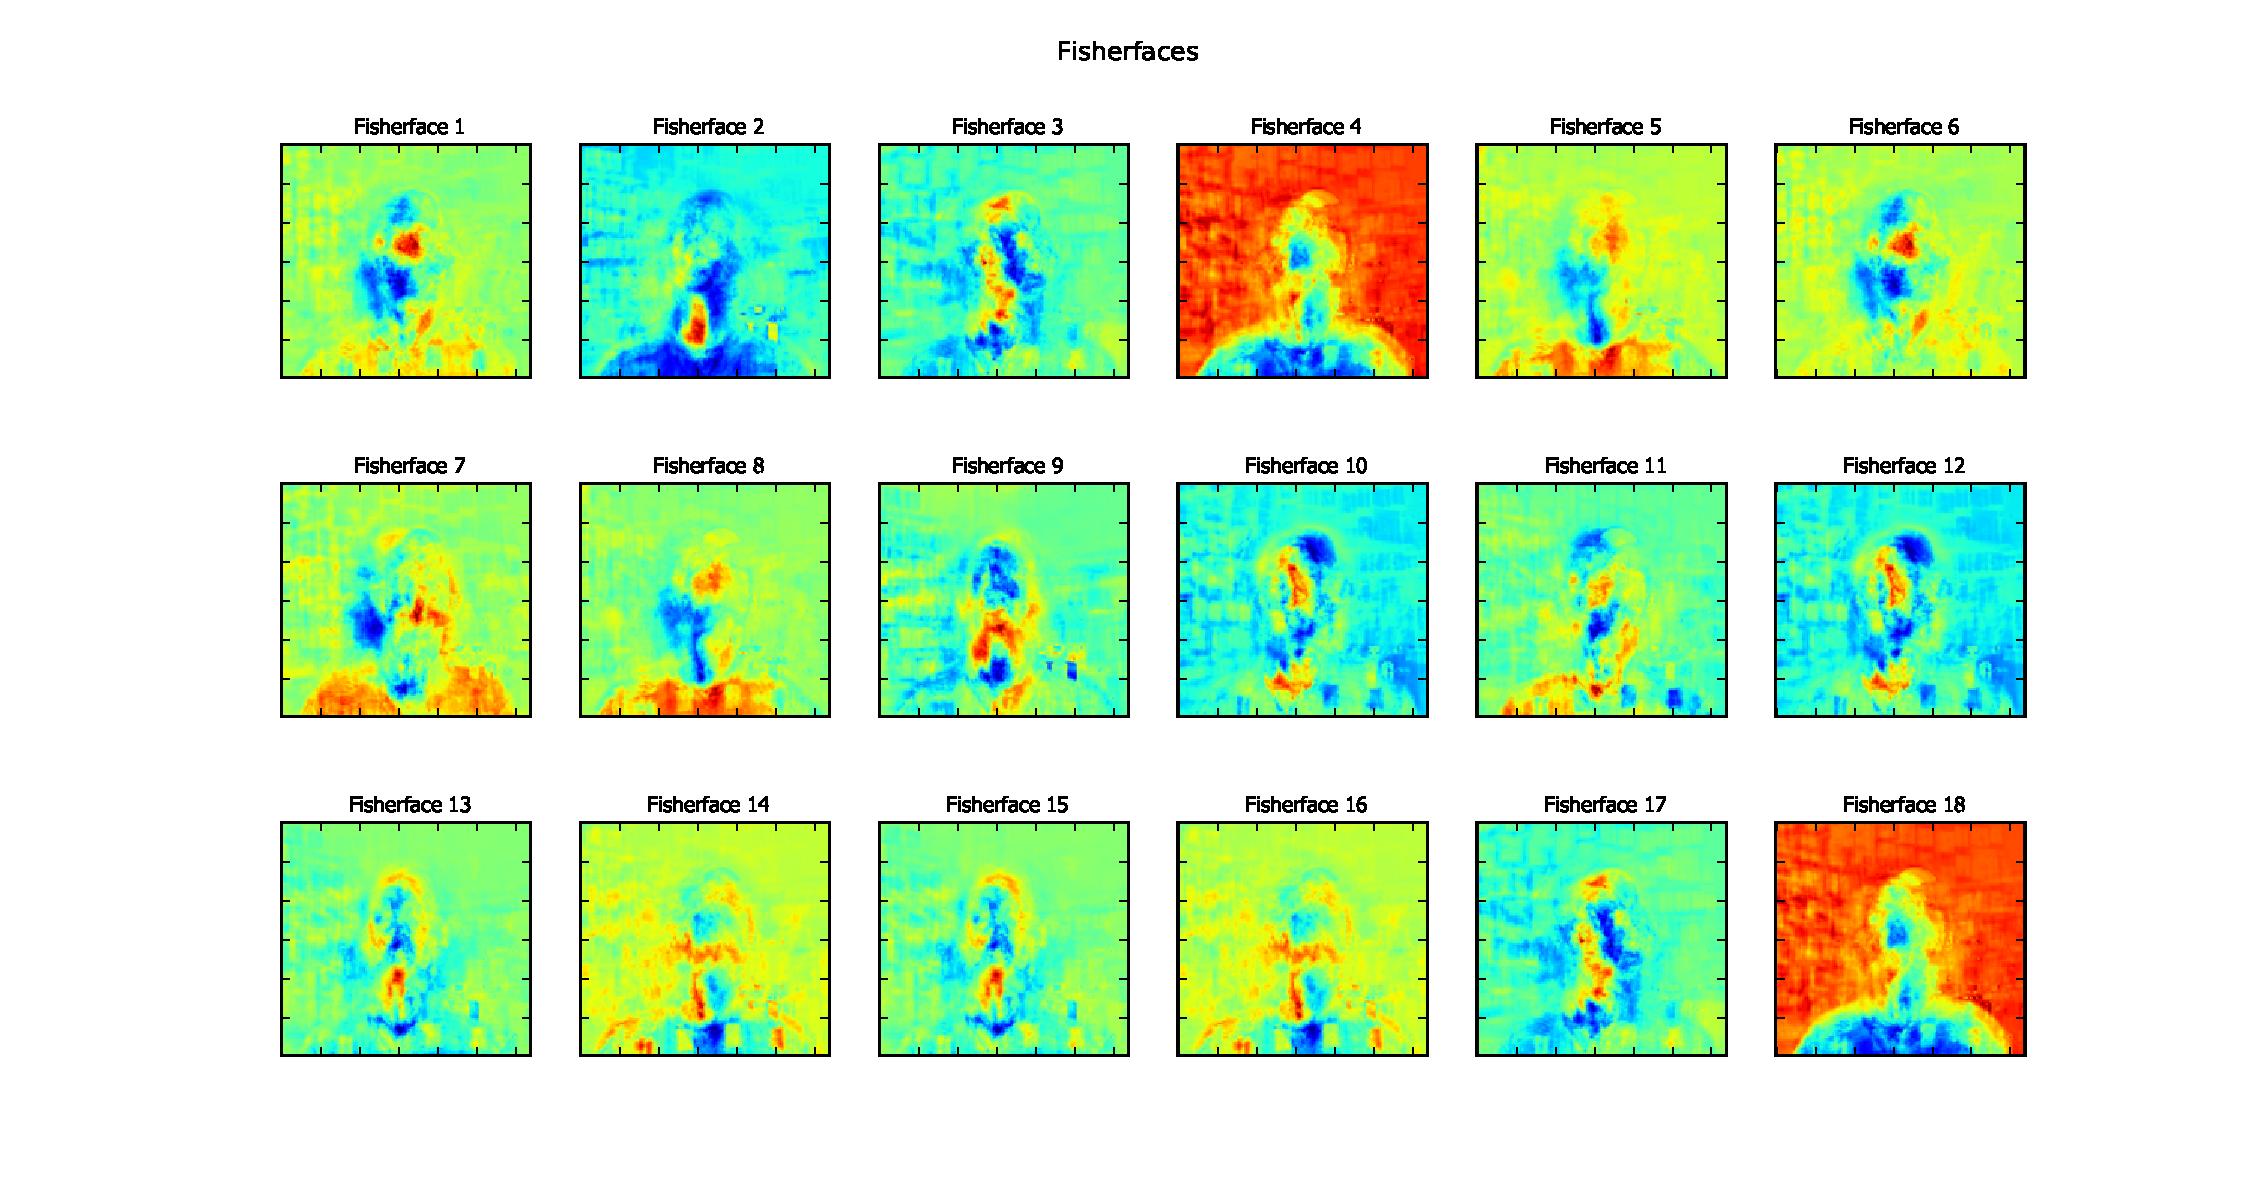
\includegraphics[width=1.0\linewidth]{fig/fisherfaces.pdf}
	\captionof{figure}{The first 18 Fisherfaces.}
	\label{fig:fisherfaces}
\end{minipage}

LDA, like PCA, performs supervised dimensionality reduction, and Fisherfaces are the subspace consisting of most discriminant bases.  Unlike eigenfaces, Fisherfaces highlight the differences among classes\cite{bel97}. 

\section{Experiment}

\subsection{Setup}

The dataset that we use for this study can be downloaded online\footnote{\url{http://www.cs.cmu.edu/afs/cs.cmu.edu/project/theo-8/faceimages/faces/}}. The data consists of about 2000 images containing four different characteristic features: person, orientation, mood and eyewear.  The images are 8-bit grayscale images with centered faces and a uniform background.  We forgo any preprocessing and use the images as they are. Also, the dataset comes with three different resolutions.

We train our algorithm on the training set, which corresponds to 60\% of our dataset, and we choose classifiers for different features by running our algorithm on the validation set, 15\% of our dataset. After choosing the best performing classifier for each feature on the validation set, we run it on the test set.

We implement the PCA algorithm in Python\footnote{Python 2.7.5}. In our dataset we have three different resolutions ($120\times128$, $60\times64$, and $30\times32$) for the same set of images.  

\subsection{Results}

\begin{minipage}{0.45\linewidth}
	\centering
	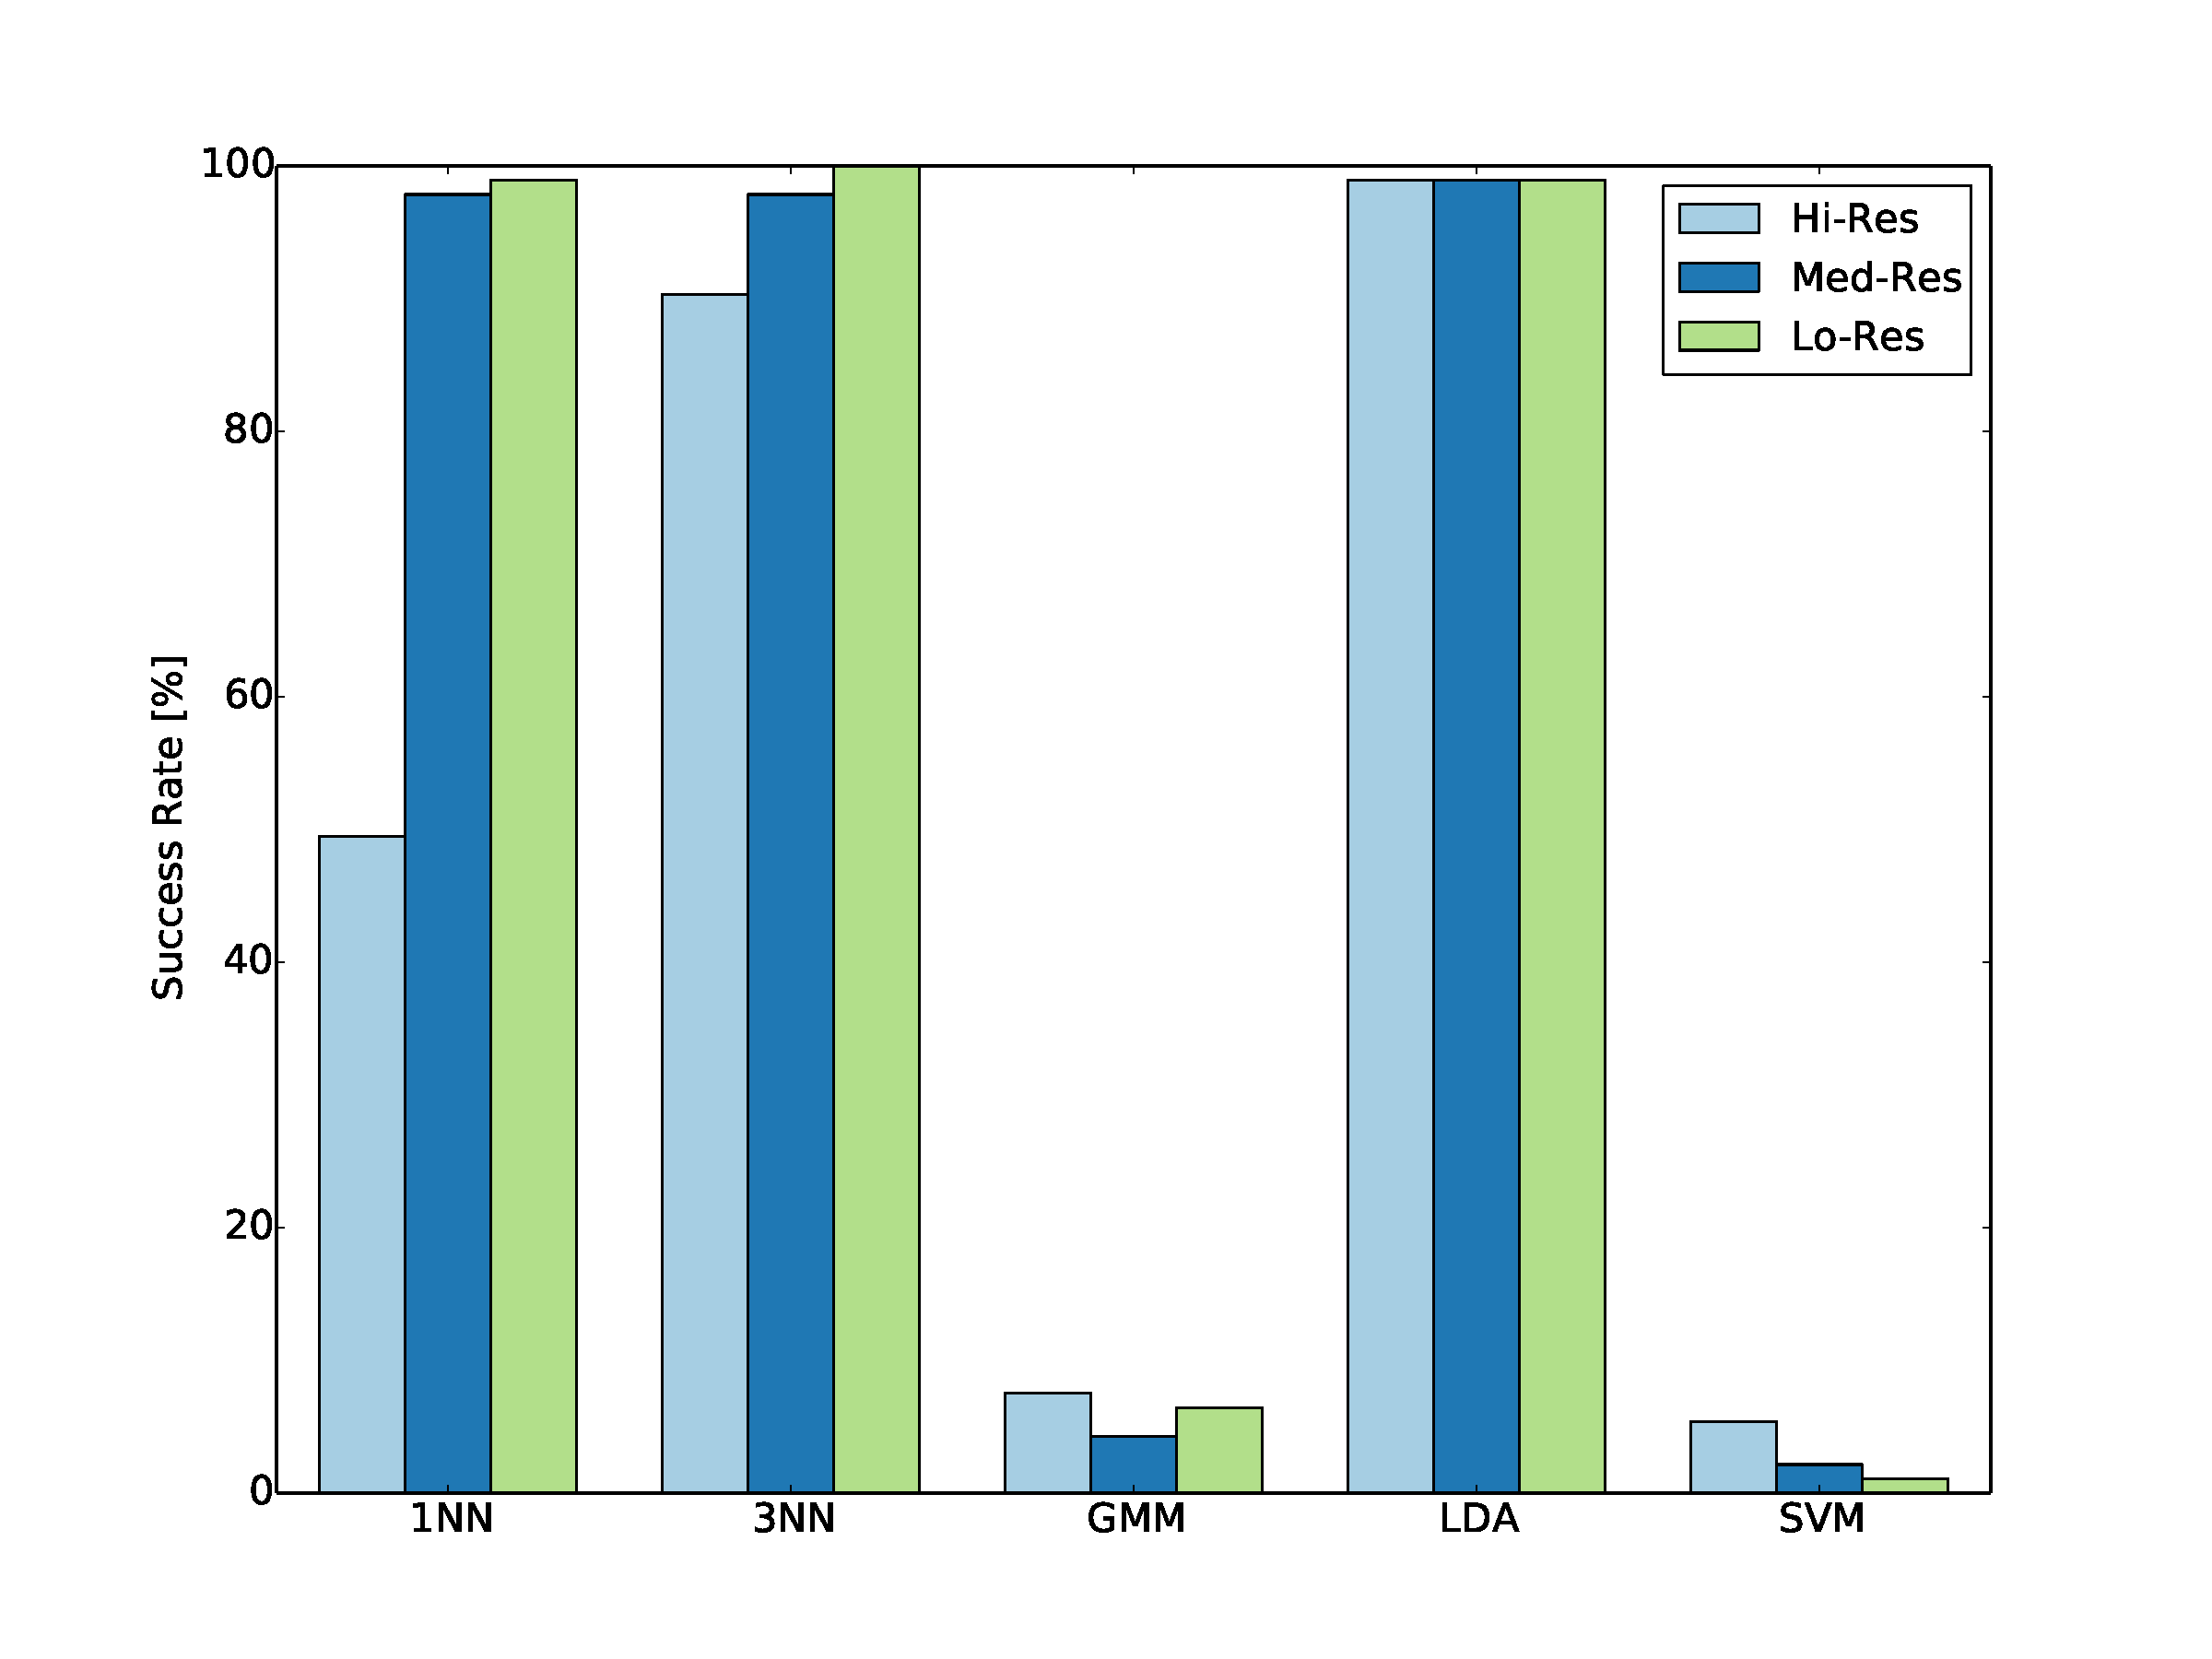
\includegraphics[height=2in]{fig/person.pdf}
	\captionof{figure}{Success rates for predicting the person.}
	\label{fig:person}
\end{minipage}
\hfill
\begin{minipage}{0.45\linewidth}
	\centering
	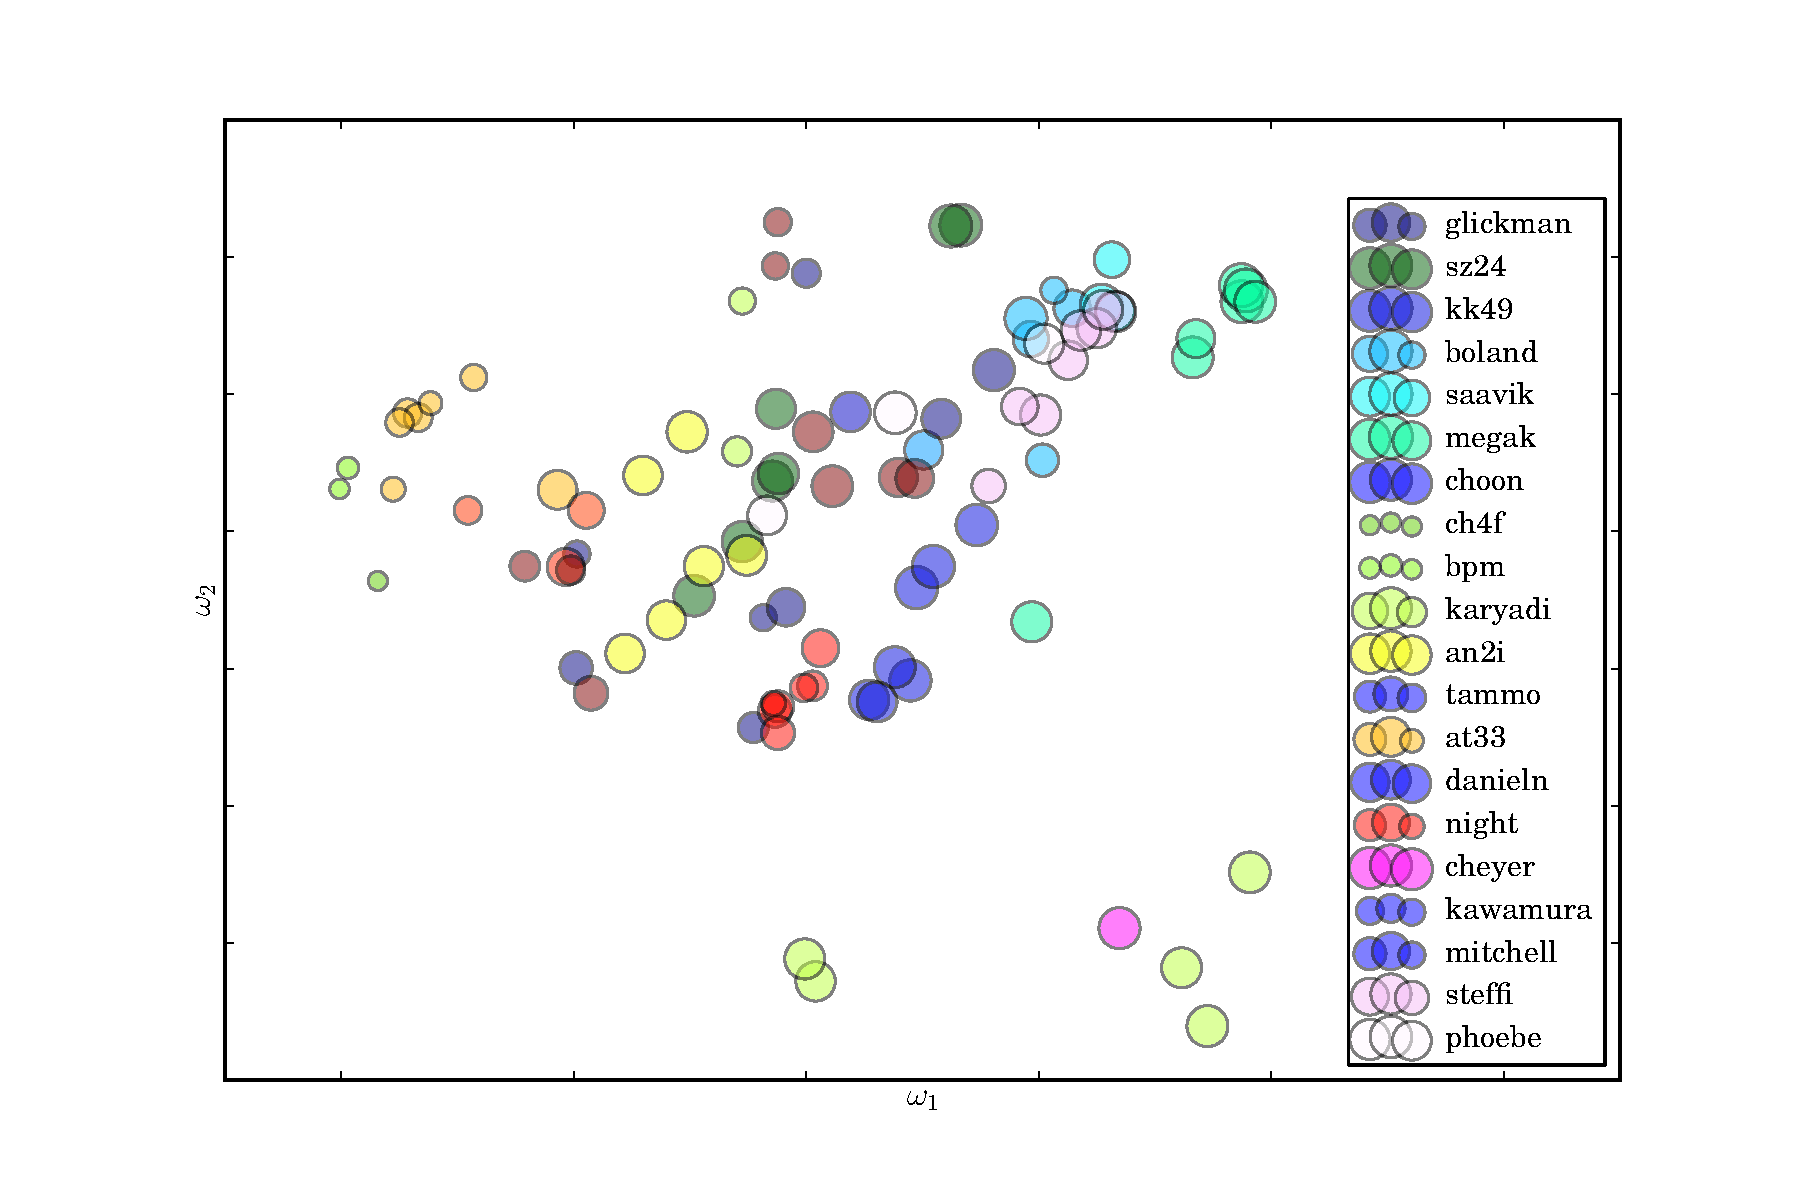
\includegraphics[height=2in]{fig/person_scatter.pdf}
	\captionof{figure}{Scatter plot of two dominant principal components for validation set.}
	\label{fig:person_scat}
\end{minipage}

Each image is identified based on the algorithm used and success rates are shown in Figure \ref{fig:person}.  The success rate is defined as the number of correct label classifications over the total number of images in the data subset, validation set here.  LDA's performance is uniform on all different resolutions even though the highest successs rate is for 3NN with 100\% on the low resolution images.  In light of this fact we choose LDA as the classifier for person on the test set.  Figure \ref{fig:person_scat} clearly shows the clustering of faces in the validation data. The size of the marker is proportional to the total Mahalanobis distance from the trained characteristic weights.

\begin{minipage}{0.45\linewidth}
	\centering
	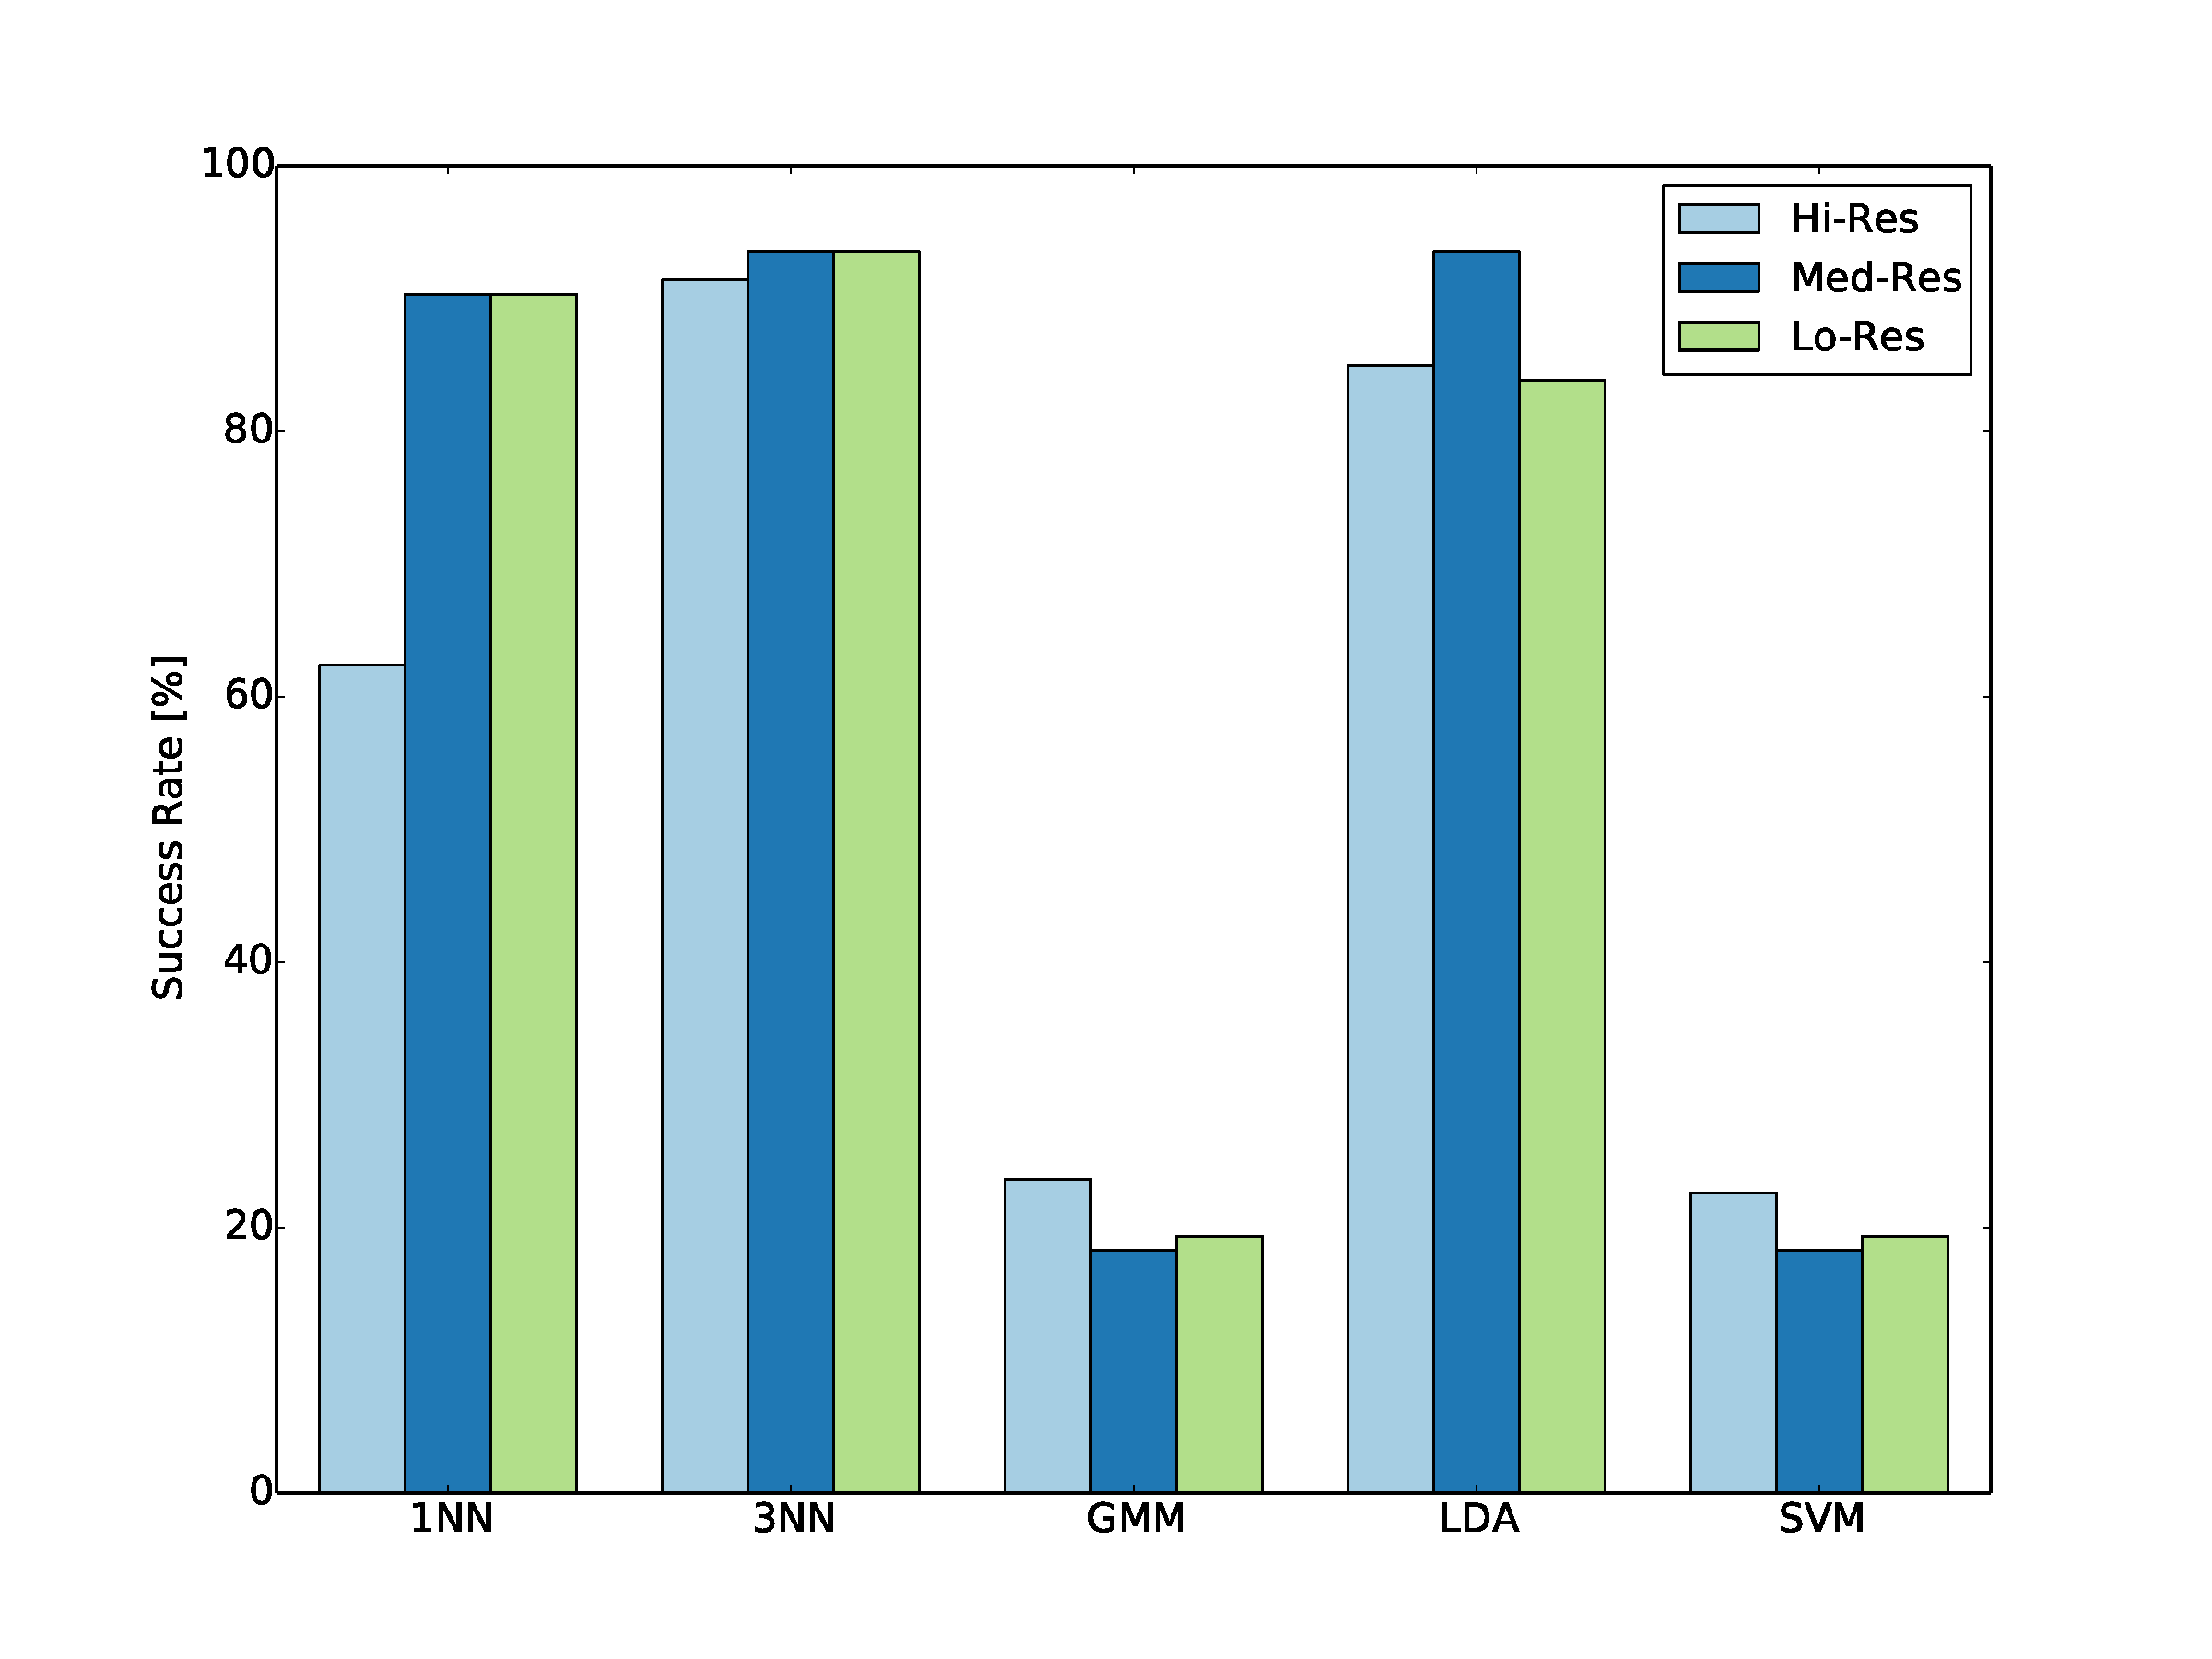
\includegraphics[height=2in]{fig/orientation.pdf}
	\captionof{figure}{Success rates for predicting the orientation.}
	\label{fig:orientation}
\end{minipage}
\hfill
\begin{minipage}{0.45\linewidth}
	\centering
	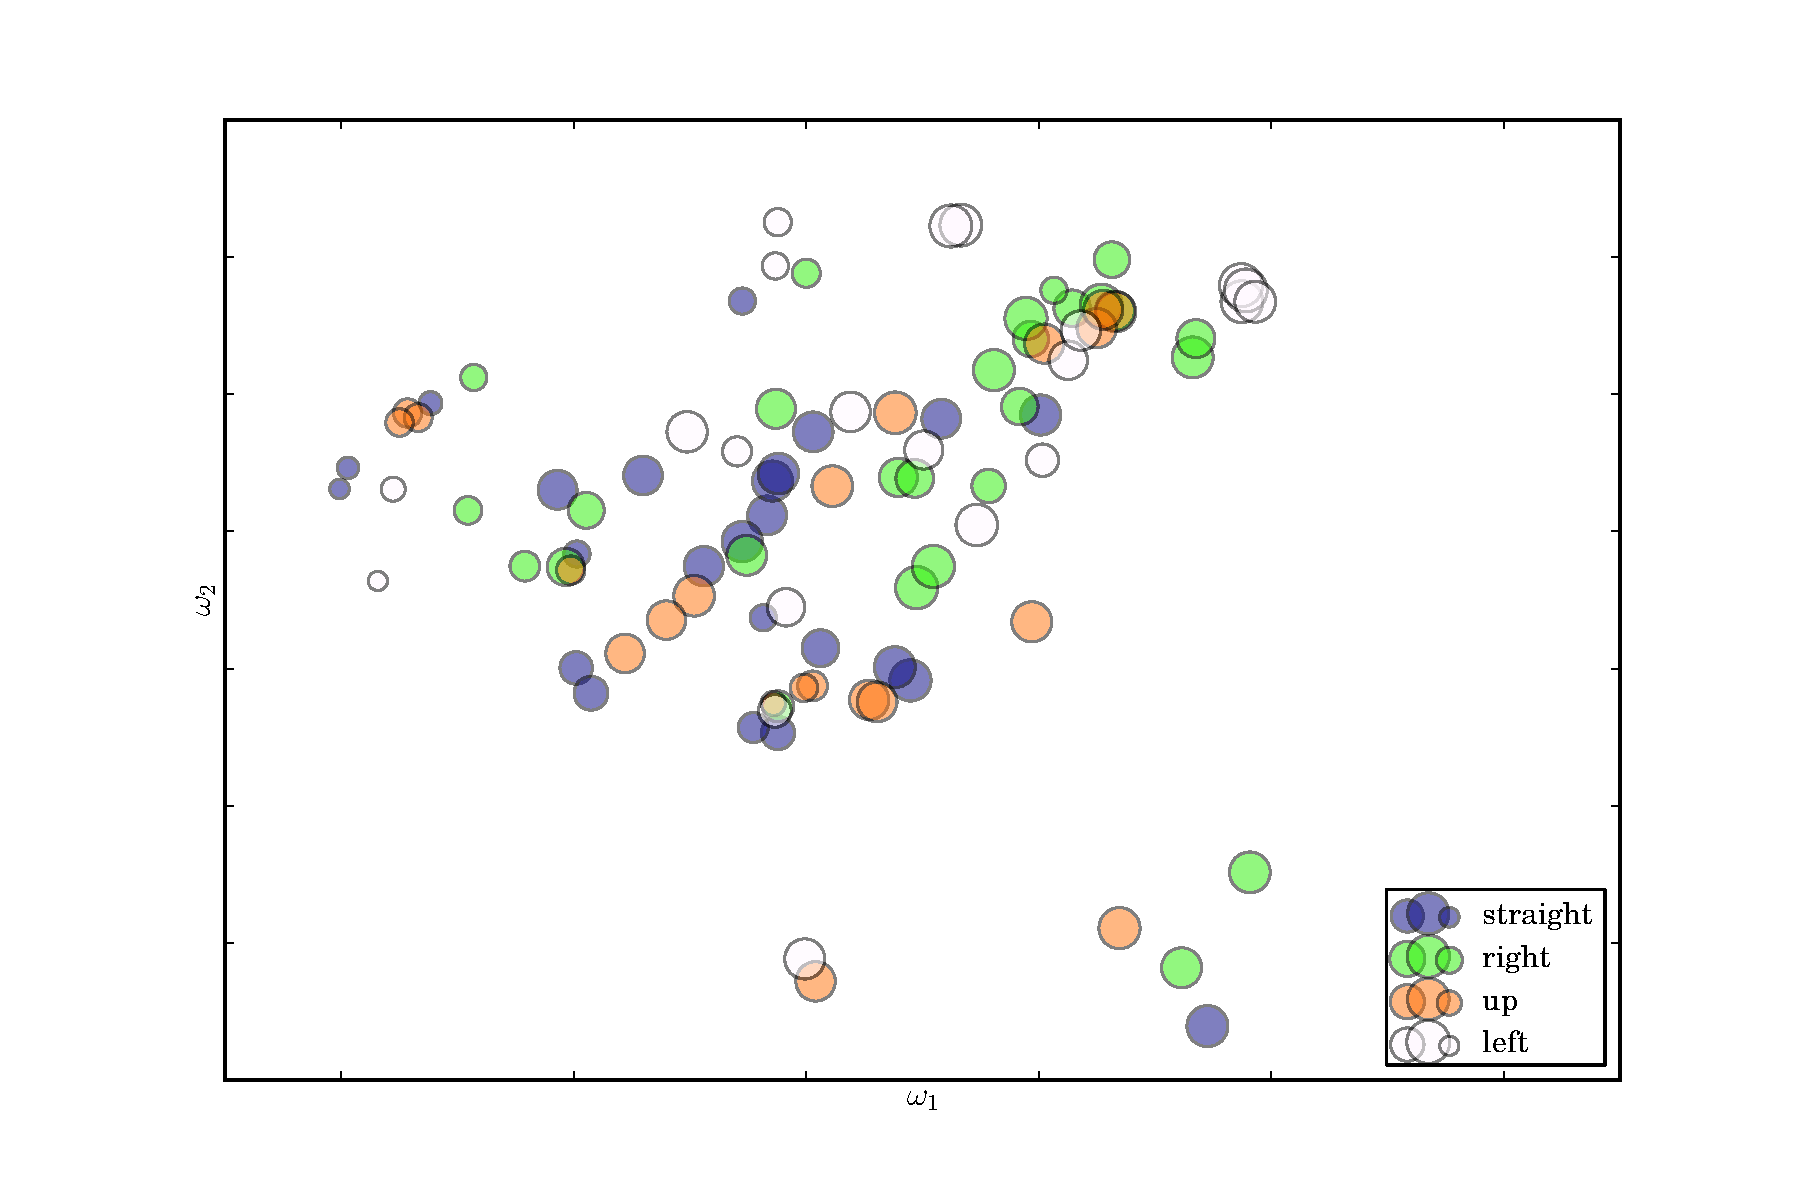
\includegraphics[height=2in]{fig/orientation_scatter.pdf}
	\captionof{figure}{Scatter plot of two dominant principal components for validation set.}
	\label{fig:orientation_scat}
\end{minipage}

In Figure \ref{fig:orientation} it can be seen that 3NN performs best across the board.  Naturally, we choose 3NN as the classifier for predicting orientation on the test data.

\begin{minipage}{0.45\linewidth}
	\centering
	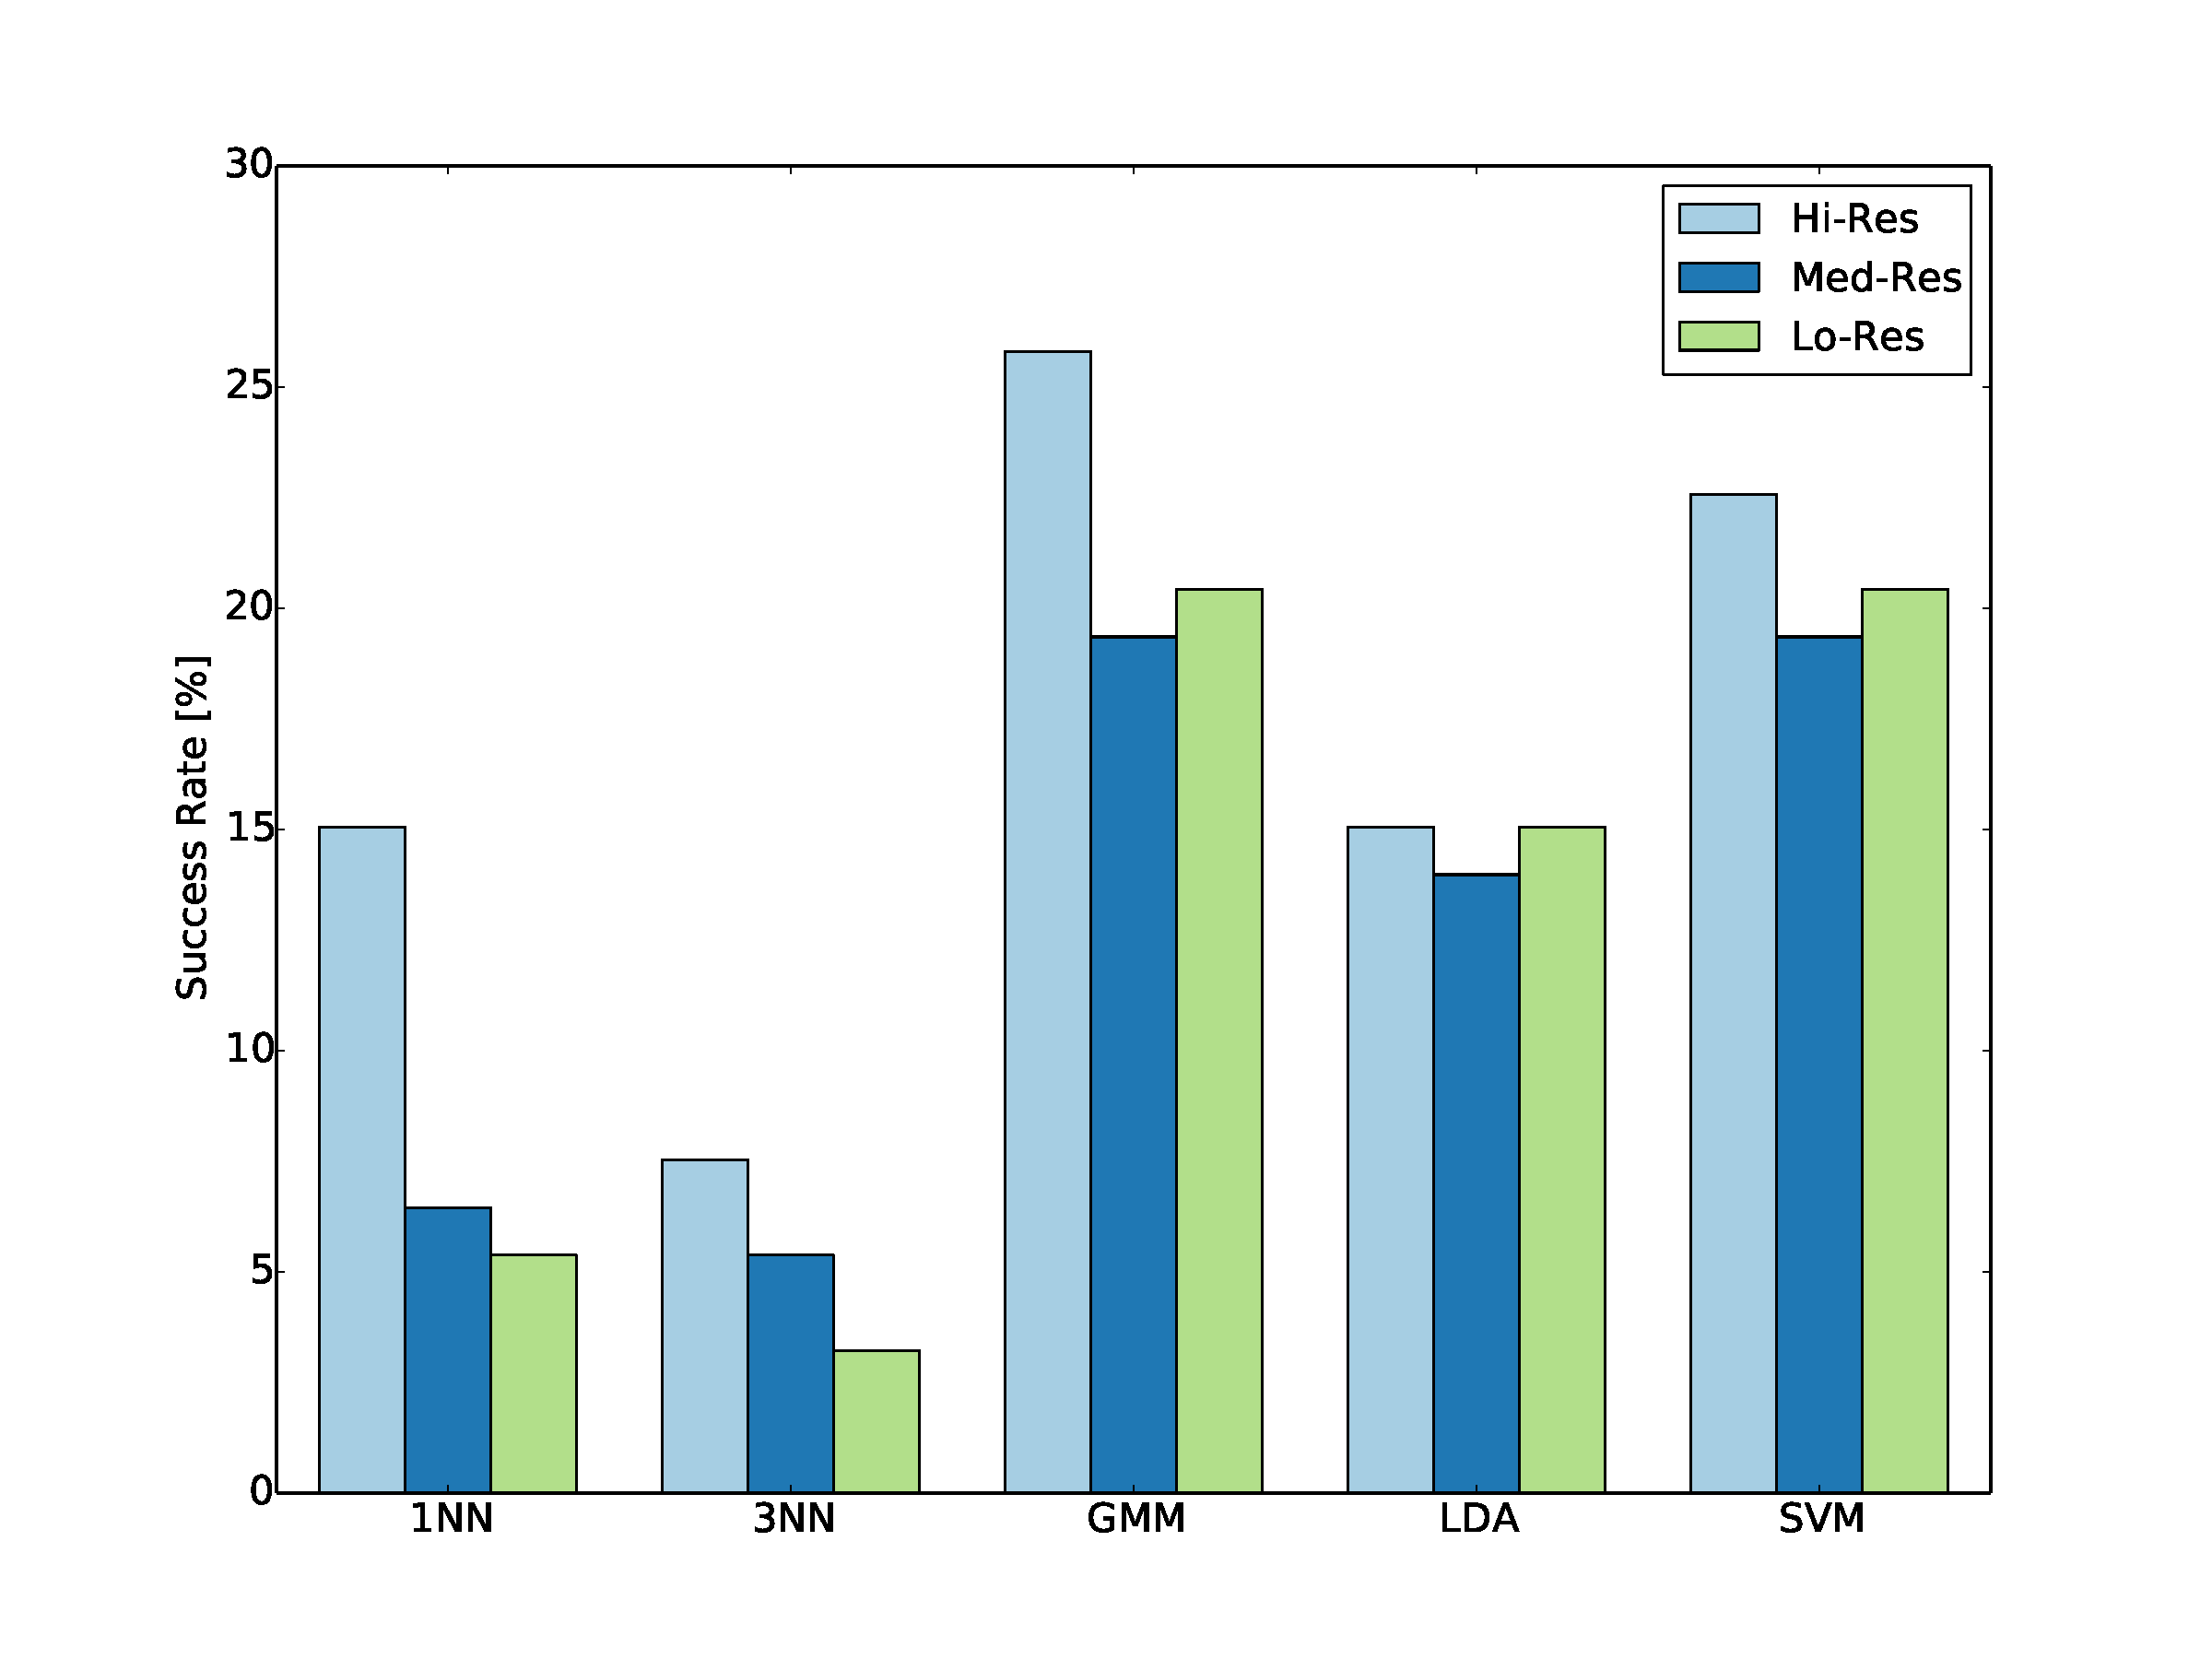
\includegraphics[height=2in]{fig/mood.pdf}
	\captionof{figure}{Success rates for predicting the mood.}
	\label{fig:mood}
\end{minipage}
\hfill
\begin{minipage}{0.45\linewidth}
	\centering
	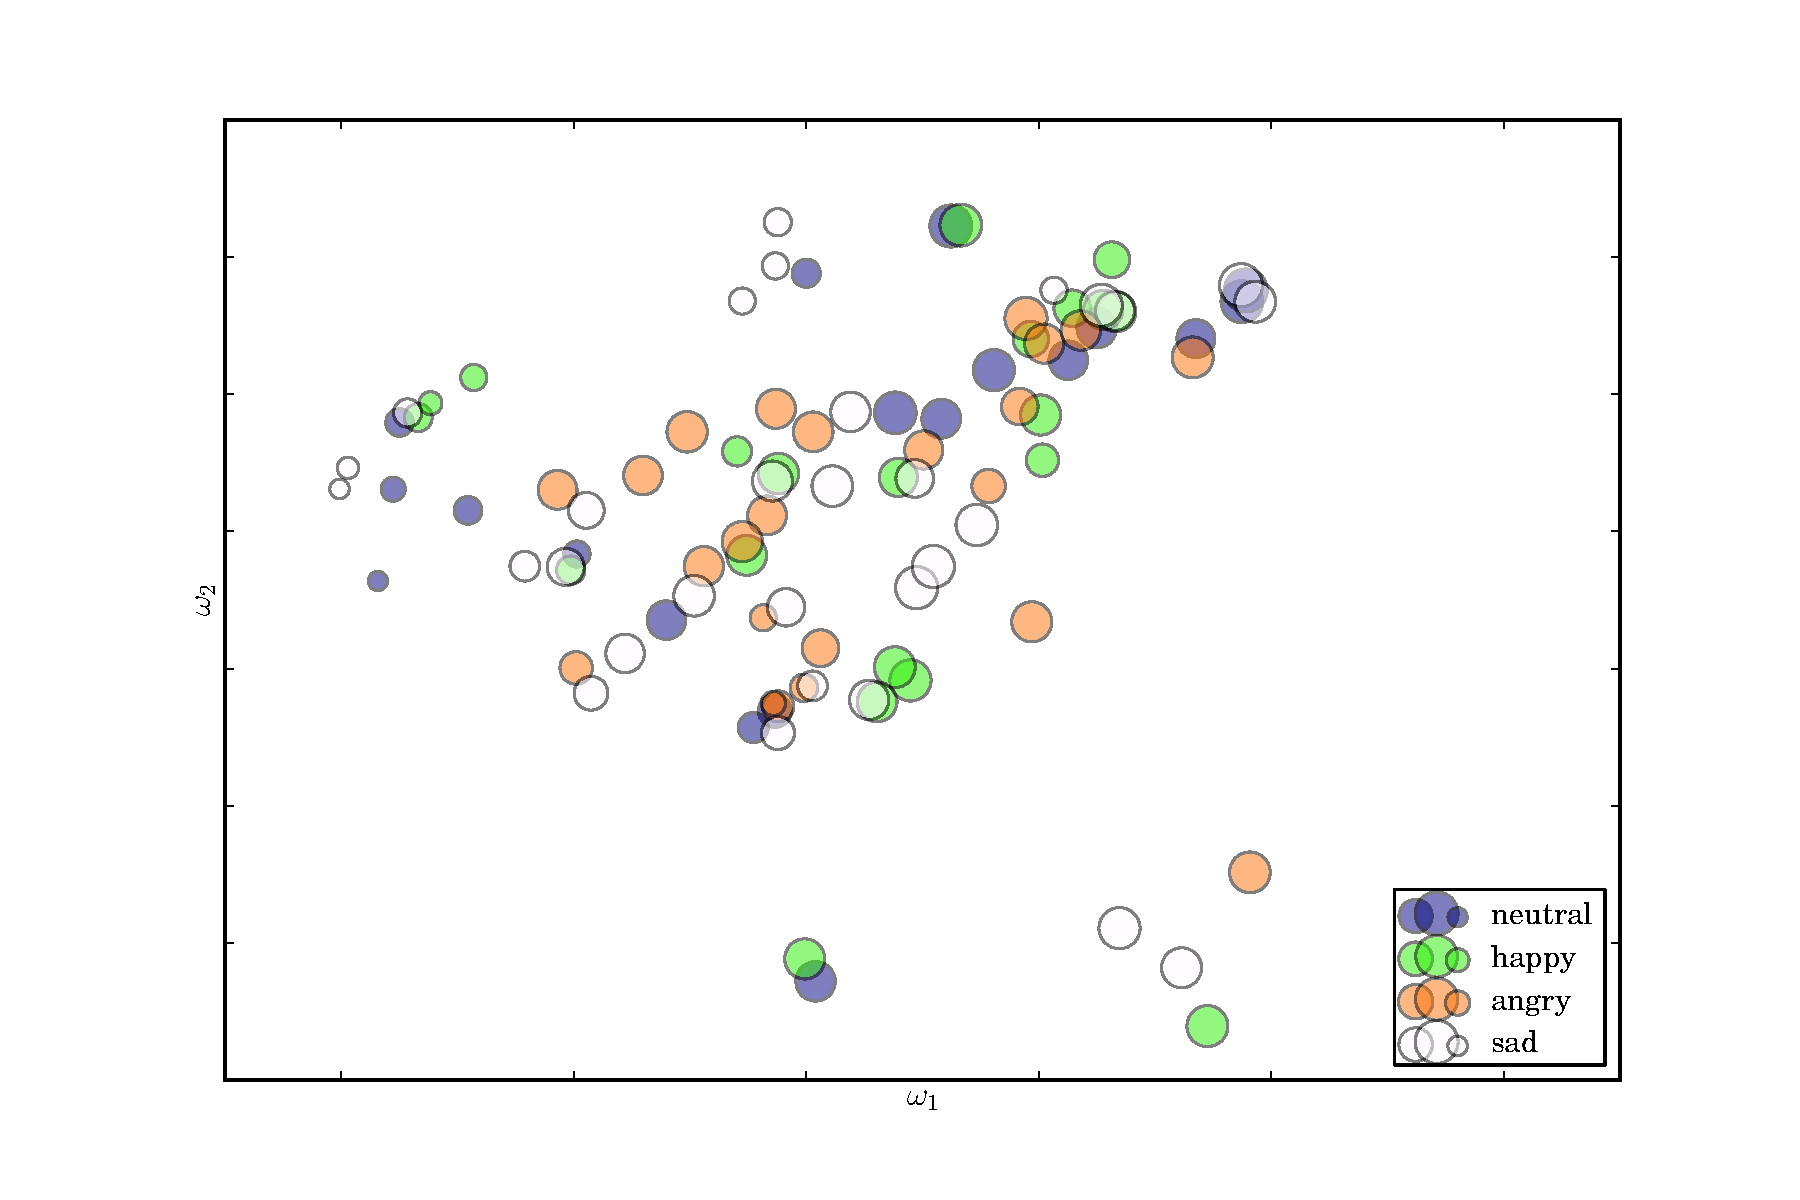
\includegraphics[height=2in]{fig/mood_scatter.pdf}
	\captionof{figure}{Scatter plot of two dominant principal components for validation set.}
	\label{fig:mood_scat}
\end{minipage}

Notice in Figure \ref{fig:mood} that most of the classifiers perform worse than random on predicting the mood.  Still GMM and SVM perform with less bias than the other the other classifiers, so we select GMM as the classifier for mood.  The reason for this can be partially explained by Figure \ref{fig:mood_scat} in which clustering among classes is absent.

\begin{minipage}{0.45\linewidth}
	\centering
	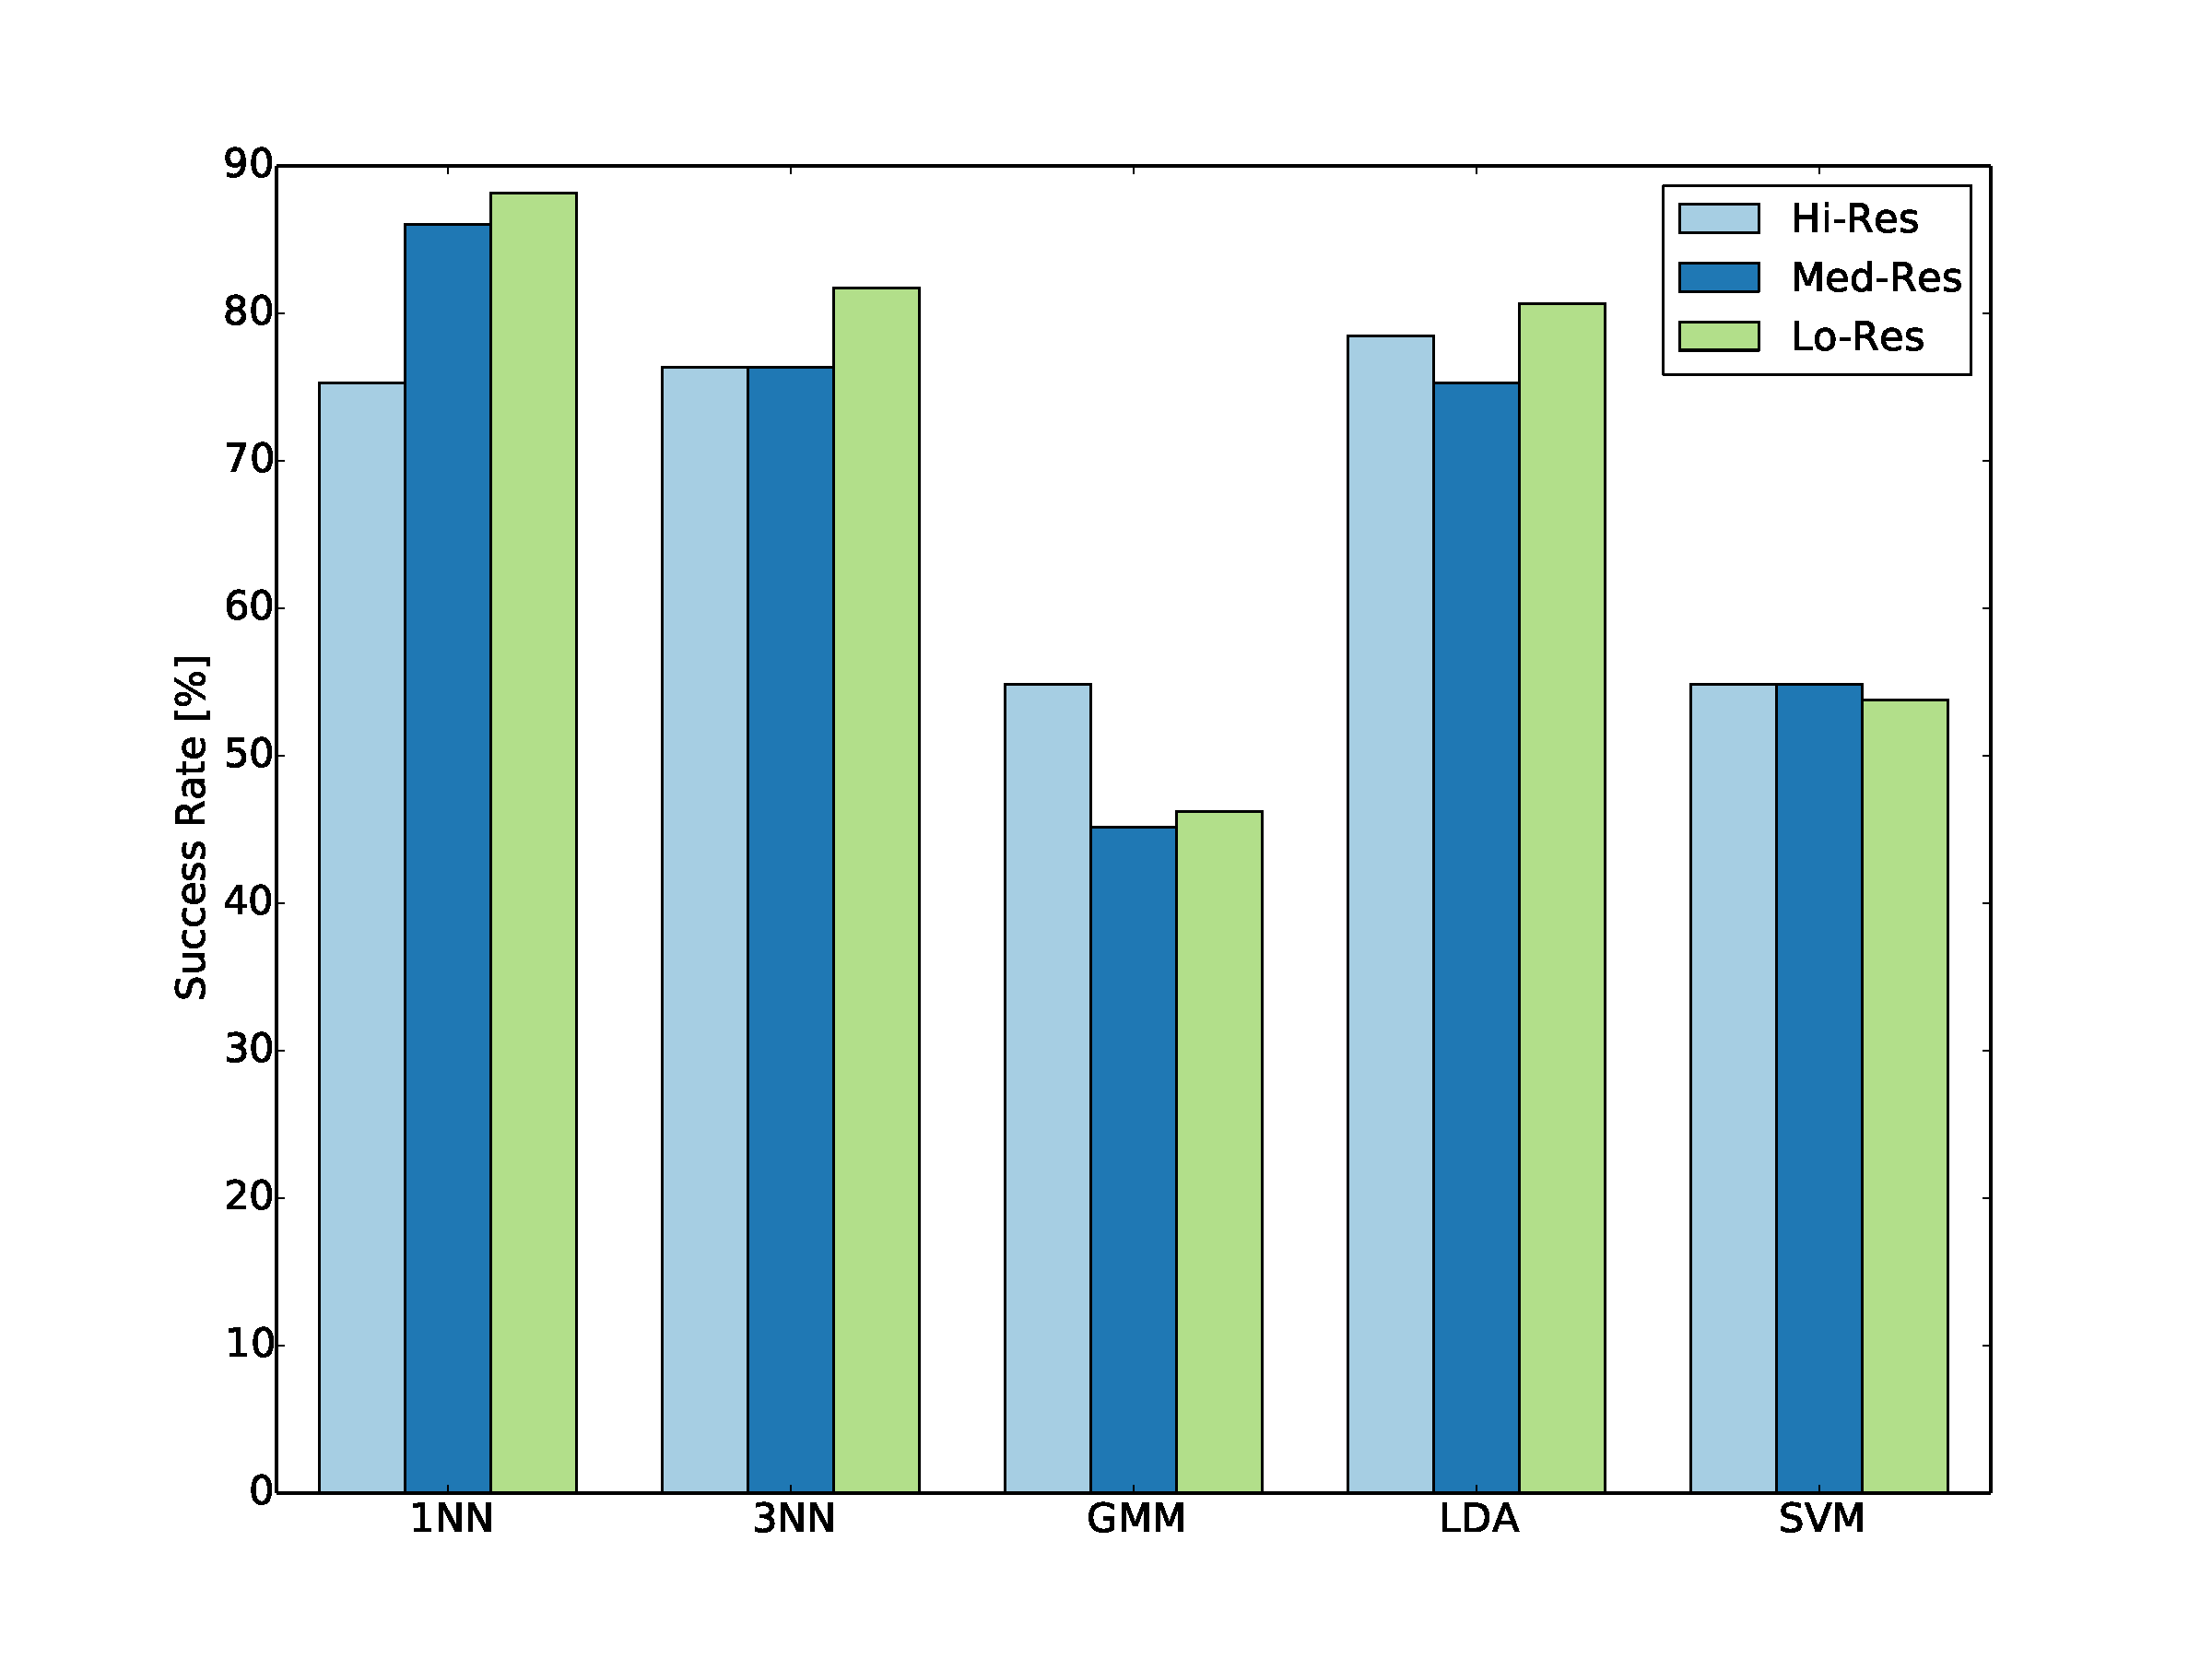
\includegraphics[height=2in]{fig/eyewear.pdf}
	\captionof{figure}{Success rates for predicting the eyewear.}
	\label{fig:eyewear}
\end{minipage}
\hfill
\begin{minipage}{0.45\linewidth}
	\centering
	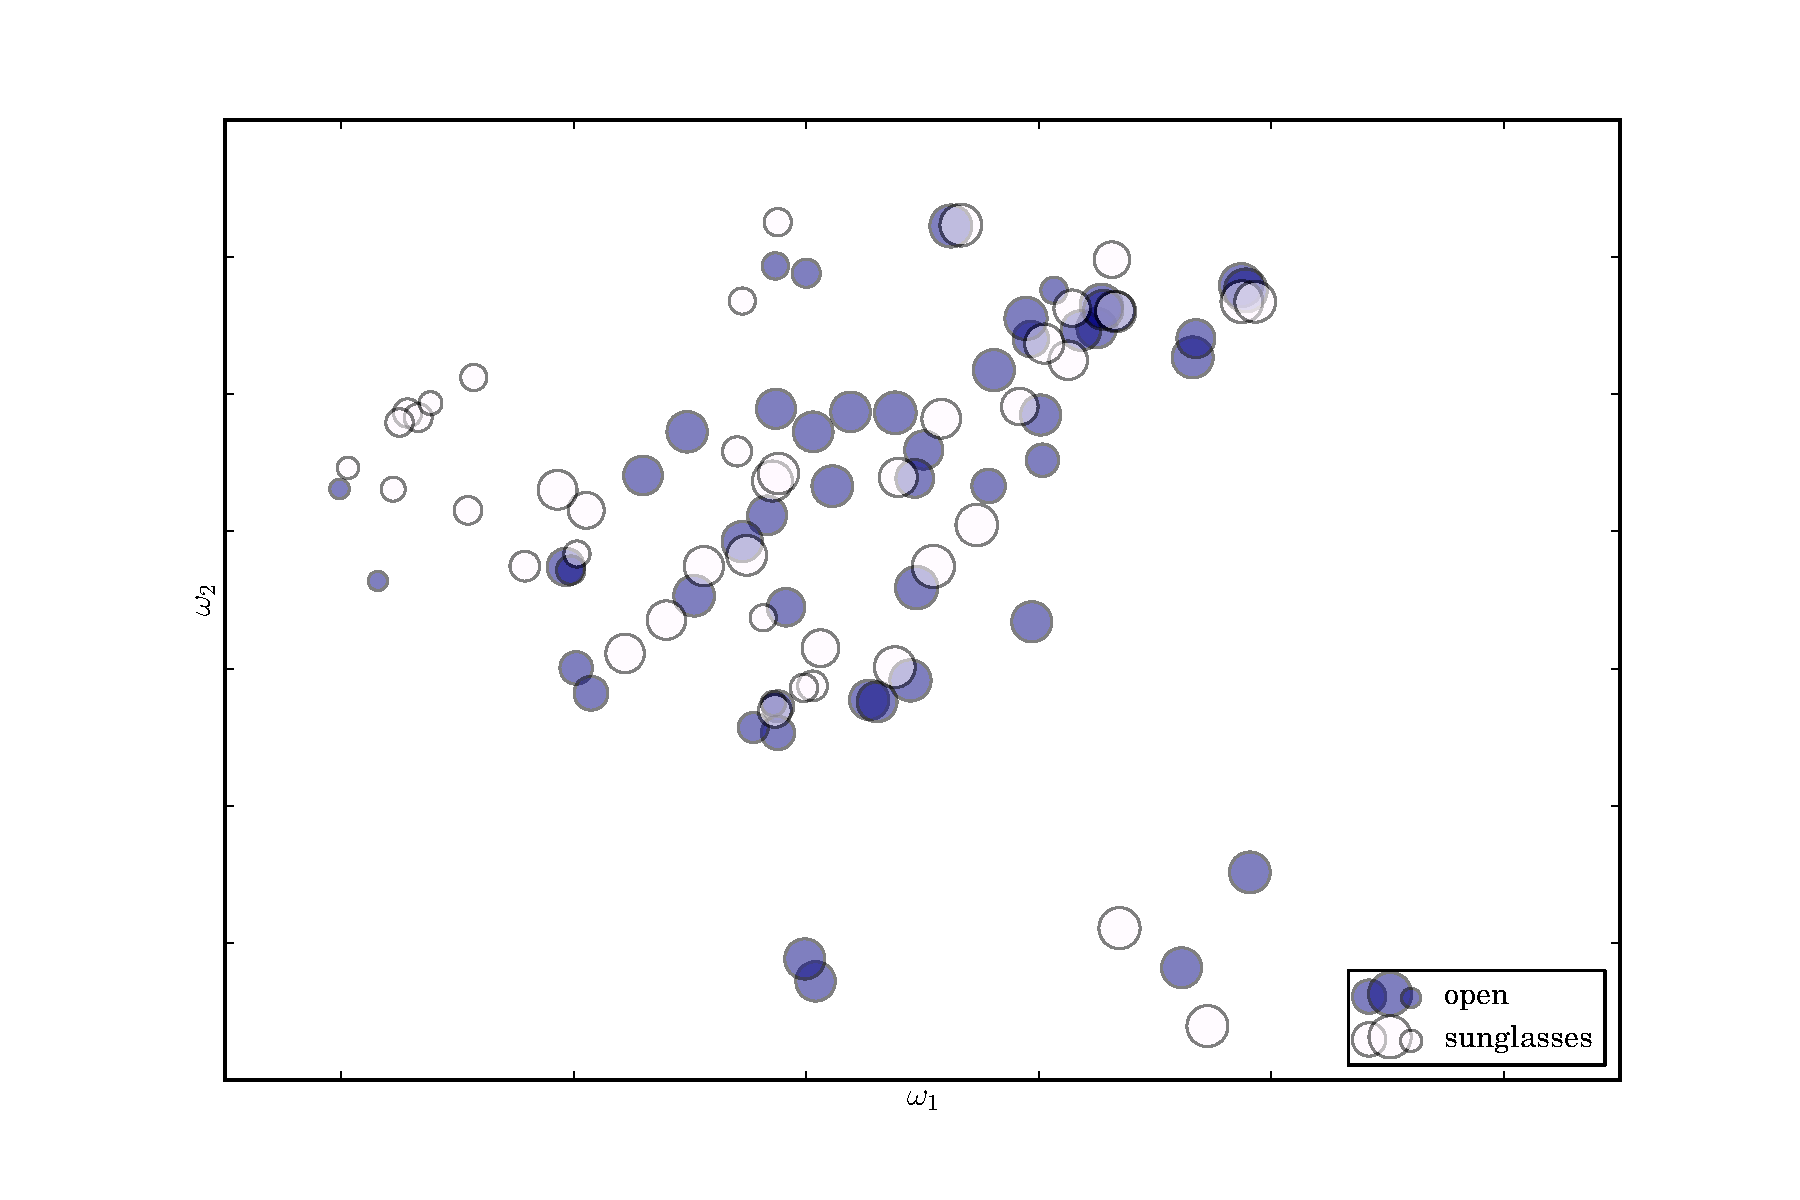
\includegraphics[height=2in]{fig/eyewear_scatter.pdf}
	\captionof{figure}{Scatter plot of two dominant principal components for validation set.}
	\label{fig:eyewear_scat}
\end{minipage}

Figure \ref{fig:eyewear} shows that 1NN is the most successful classifier for detecting eyewear, so we choose 1NN to use on the test data. 

\begin{minipage}{\linewidth}
	\centering
	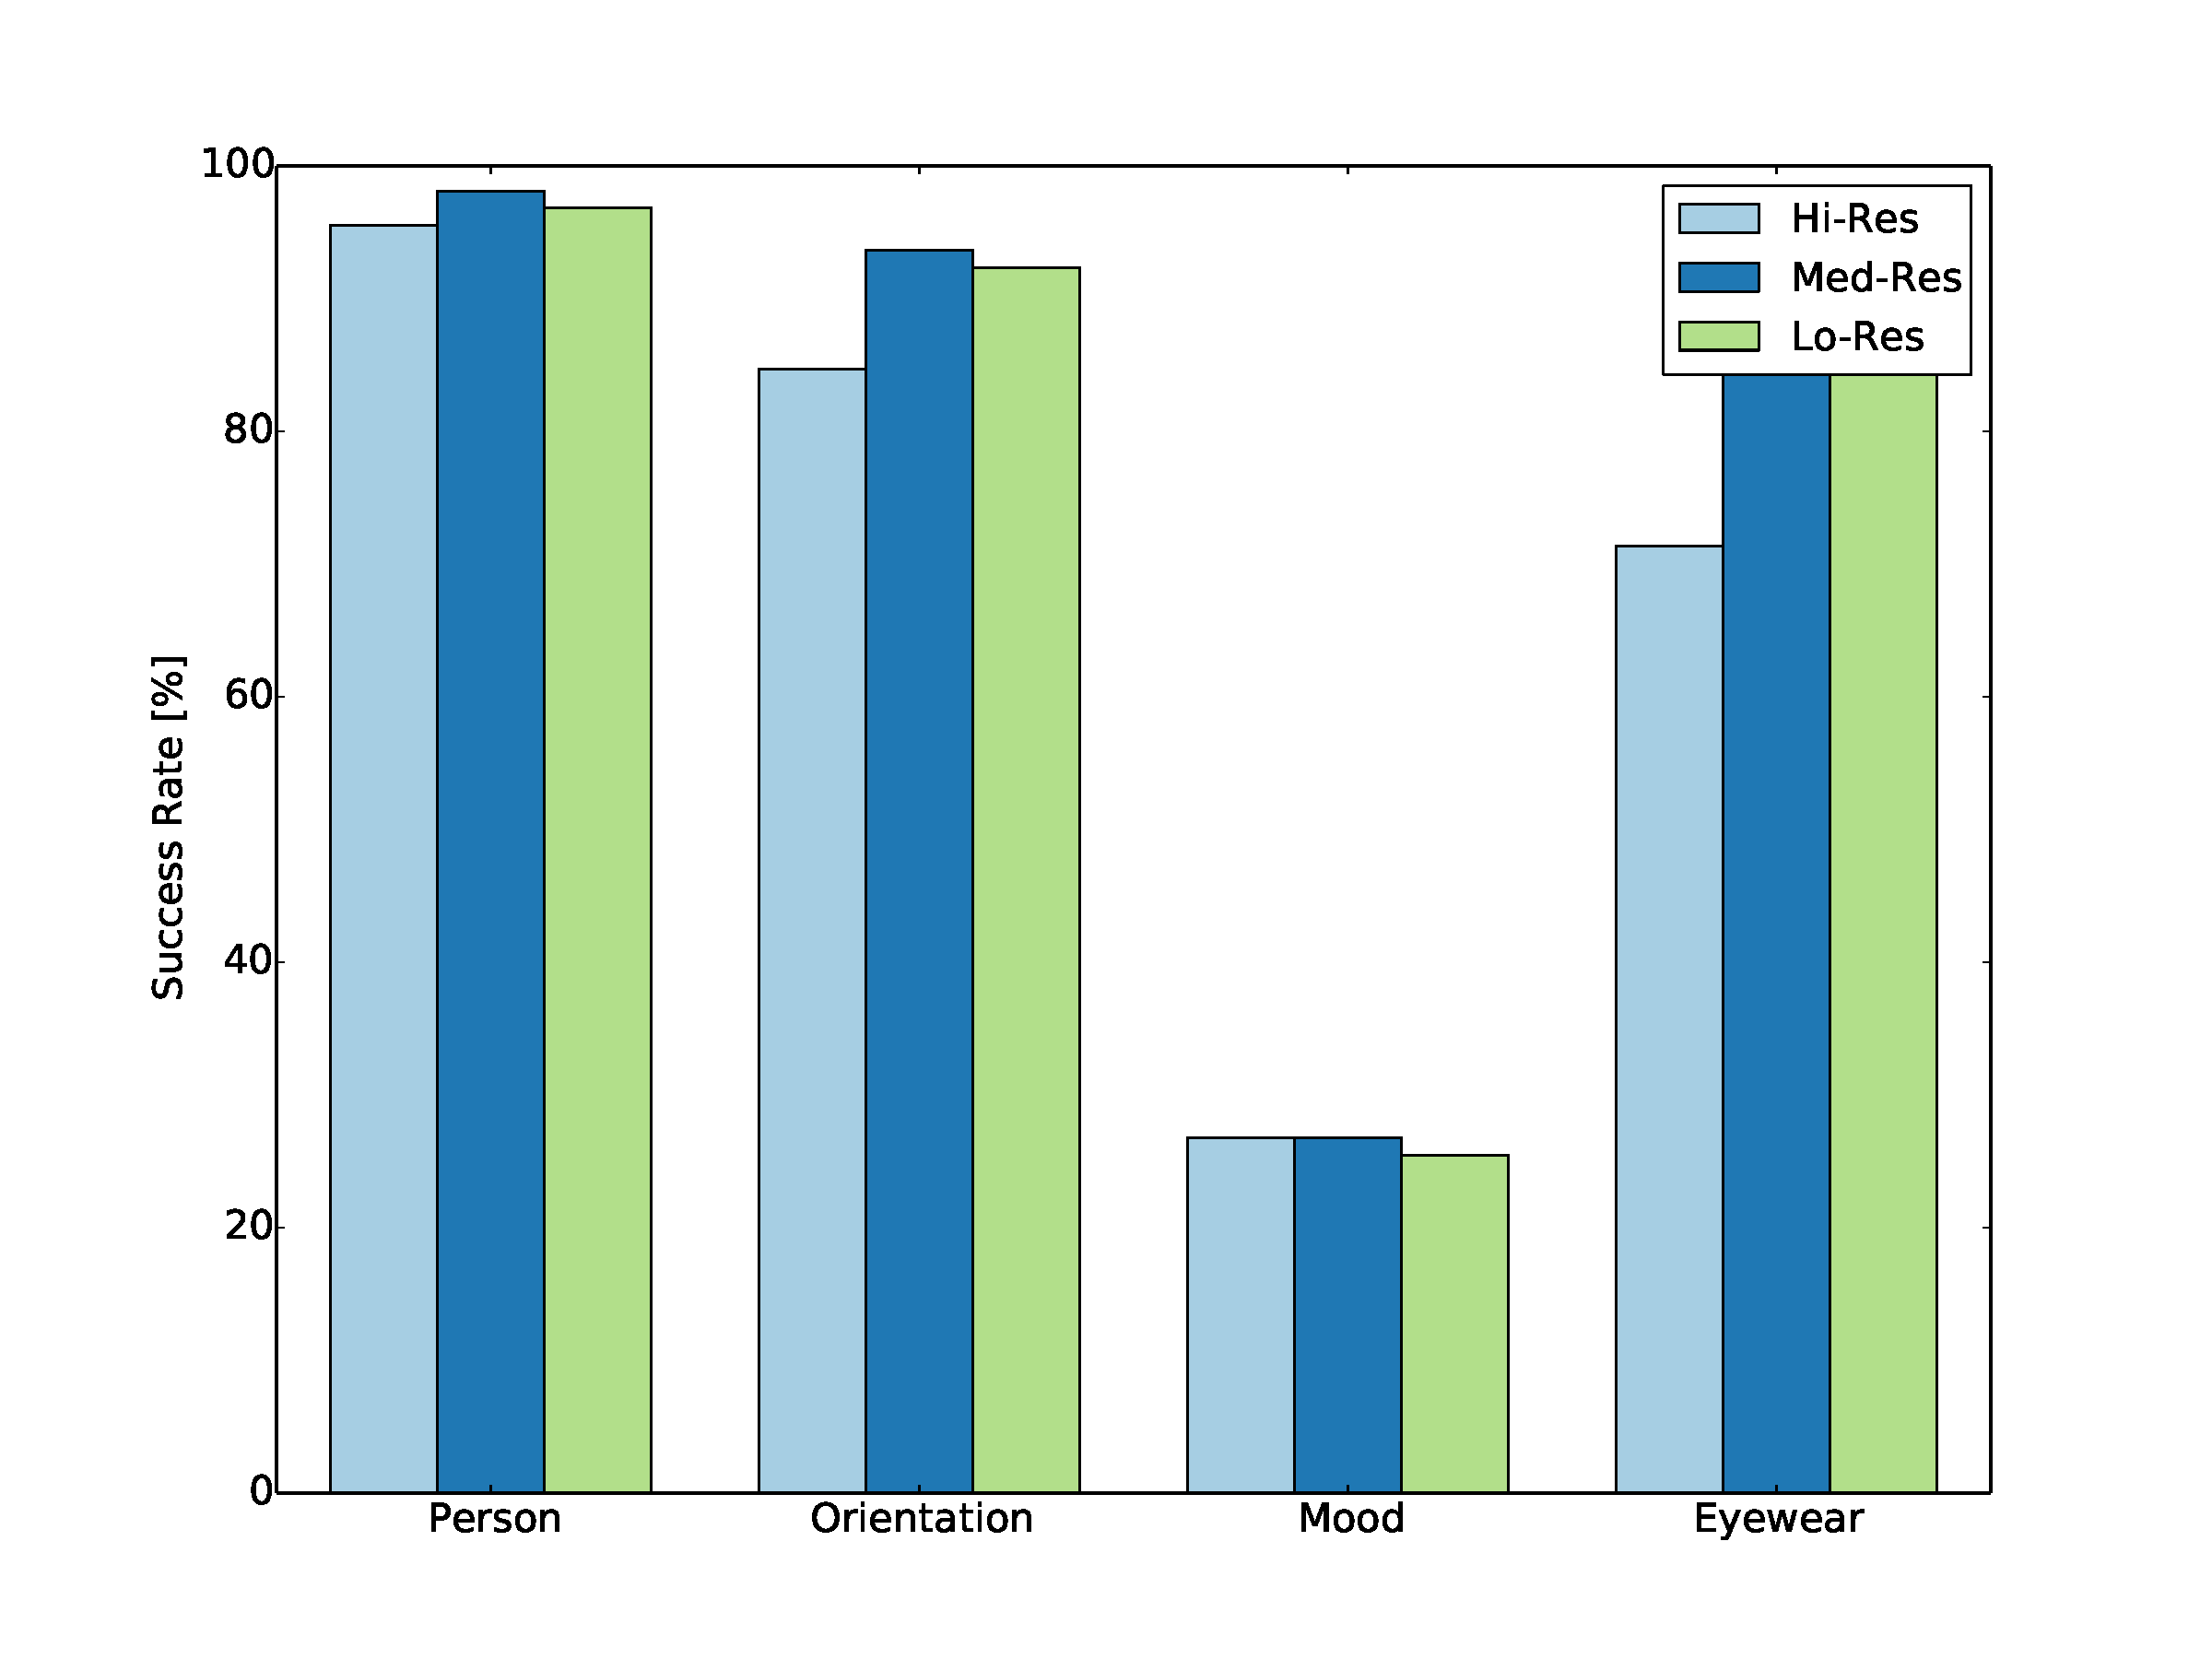
\includegraphics[width=\linewidth]{fig/test.pdf}
	\captionof{figure}{Success rates for the test data.}
	\label{fig:test}
\end{minipage}

As can be seen in Figure \ref{fig:test}, we achieve more than 70\% success rates in predicting person, orientation, and eyewear for all resolutions.  All of our classifiers perform worse than random in predicting mood. However, GMM performs as well as random.

\section{Conclusion}

In this study we examine the performance of different classifiers on predicting different facial features. We find that some classifiers perform better compared to others on each facial feature.  Nonetheless, we cannot successfully predict mood with any of the tested classifiers.  

The results show that there are better classifiers for different features.  Classifier selection should be done using validation data to achieve the best performance.  

\bibliography{rmf}{}
\bibliographystyle{unsrt}

\end{document} 
